\documentclass[11pt]{article}
\usepackage{geometry}
\geometry{letterpaper}

\usepackage{graphicx}
\usepackage{amssymb}
\usepackage{epstopdf}
\usepackage{natbib}
\usepackage{amssymb, amsmath}
\usepackage{listings}
\usepackage[final]{pdfpages}
\usepackage[framed,numbered,autolinebreaks,useliterate]{mcode}
\usepackage{tikz}
\usepackage{subfig}
\usepackage[underline=true,rounded corners=false]{pgf-umlsd}
\usepackage{tikz-uml}
\usepackage{url}
\usepackage{float}
\usetikzlibrary{mindmap}

\lstset{language=matlab}
\lstset{breaklines}
\lstset{extendedchars=false}
\DeclareGraphicsRule{.tif}{png}{.png}{`convert #1 `dirname #1`/`basename #1 .tif`.png}

%\title{Title}
%\author{Name 1, Name 2}
%\date{date}

\begin{document}


\input{cover}
\newpage

%%%%%%%%%%%%%%%%%%%%%%%%%%%%%%%%%%%%%%%%%%%%%%%%%

\newpage
\section*{Agreement for free-download}
\bigskip


\bigskip


\large We hereby agree to make our source code for this project freely available for download from the web pages of the SOMS chair. Furthermore, we assure that all source code is written by ourselves and is not violating any copyright restrictions.

\begin{center}

\bigskip


\bigskip


\begin{tabular}{@{}p{3.3cm}@{}p{6cm}@{}@{}p{6cm}@{}}
\begin{minipage}{3cm}

\end{minipage}
&
\begin{minipage}{6cm}
\vspace{2mm} \large Xiang Gao

\vspace{\baselineskip}

\end{minipage}
&
\begin{minipage}{6cm}

\end{minipage}
\end{tabular}


\end{center}
\newpage

%%%%%%%%%%%%%%%%%%%%%%%%%%%%%%%%%%%%%%%

% IMPORTANT
% you MUST include the ETH declaration of originality here; it is available for download on the course website or at http://www.ethz.ch/faculty/exams/plagiarism/index_EN; it can be printed as pdf and should be filled out in handwriting
% \includepdf[pages={1}]{declare.pdf}

%%%%%%%%%% Table of content %%%%%%%%%%%%%%%%%

\tableofcontents

\newpage

%%%%%%%%%%%%%%%%%%%%%%%%%%%%%%%%%%%%%%%

\section{Introduction and Motivations}
In this paper, we will investigate the modeling of peer review process. There are not many existing papers on the modeling of peer review. In 2010, Thurner \cite{thurner2010peer} implemented a simple model and argued that a small fraction of rational referee will decrease the quality of publication obviously. Francisco \cite{grimaldoproposal} implemented a model called PR-1 which is a subset of their proposed model PR-M and their experiments showed that three reviewers are enough to perform a good selection.

The author of this paper intended to extend the existing model to a new one, but due to the time limitation and the author's ability, we only implemented a small prototype. The contribution of this paper is two fold, one is to define the six building blocks for modeling peer review, these core concepts could be the foundation for further research. Another contribution is to develop a small code framework based on the six building blocks, which could be reused, extended by other researchers so as to speed up the development of programs. We do not give any detail model or implementation about peer review process, so we call this model a generalized model. This decision is to give other people who want to extend existing model or idea more flexibility.

The rest of paper is organized as follows, we first define the six building blocks for peer review, next we describe in detail about the implementation, then we show an example model based on the building blocks and code framework, at last we conclude the paper.

\section{Six Building Blocks for Modeling Peer Review}

\begin{figure}[!th]
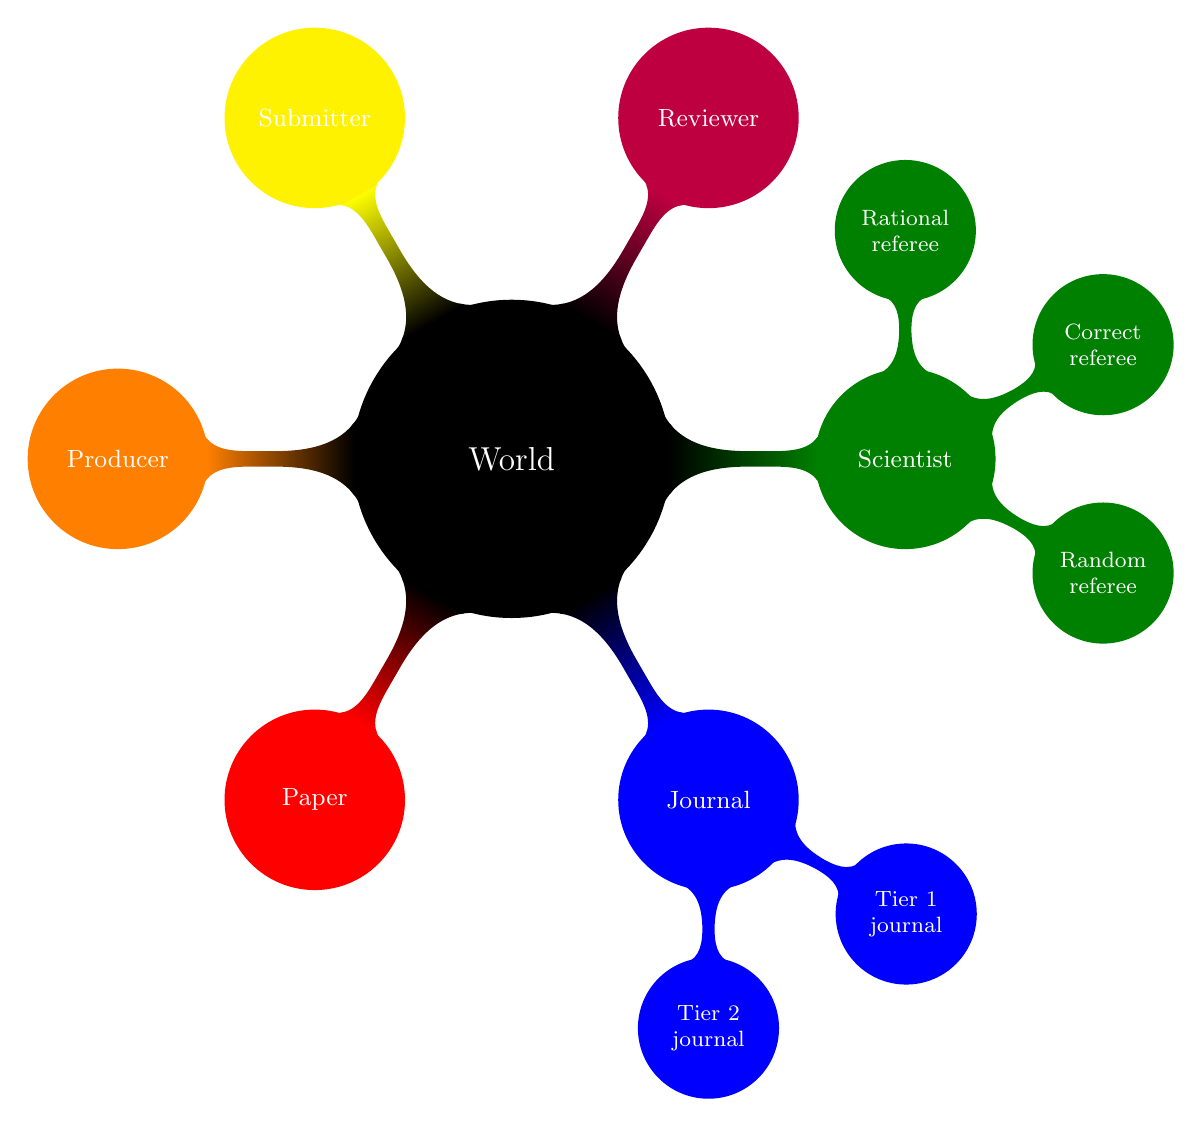
\begin{tikzpicture}[]
  \path[mindmap,concept color=black,text=white]
    node[concept] {World}
    [clockwise from=0]
    child[concept color=green!50!black] {
      node[concept] {Scientist}
      [clockwise from=90]
        child { node[concept] {Rational referee} }
        child { node[concept] {Correct referee} }
        child { node[concept] {Random referee} }
    }
    child[concept color=blue] {
    node[concept] {Journal}
    [clockwise from=-30]
      child { node[concept] {Tier 1 journal} }
      child { node[concept] {Tier 2 journal} }
    }
    child[concept color=red] { node[concept] {Paper} }
    child[concept color=orange] { node[concept] {Producer} }
    child[concept color=yellow] { node[concept] {Submitter} }
    child[concept color=purple] { node[concept] {Reviewer} };
\end{tikzpicture}
\caption{Six building blocks for modeling peer review.}
\label{fig:sbb}
\end{figure}

In the academic world, scientists, papers, and journals are three important entities. Scientists produce papers, submit papers to journals for review, after receiving the manuscript, the journal will arrange other scientists to review papers and decide if the papers are accepted, rejected, or revision. These three entities constitutes three building blocks in the peer review process.

The other three building blocks are not concrete entities, but three algorithms or methods. One is called producer, which defines the quality of the paper produced by a scientist, another one is called submitter, which decides which journal the scientist wants to submit his or her paper. The last one is named reviewer, this is the method journals use to review and accept papers.

These concepts are not new, but are extracted from existing models. Most of the existing research try to use agent based model to simulate the peer review process, when come to the implementation, they must decide the three algorithms we defined as building blocks. Different models employ different algorithms for the three algorithm building blocks and use different attributes of the three entity building blocks. Each one of the building blocks can be designed separately, and you can run a lot of experiments with differently combinations. This will result in a lot of work to find the best method to implement the peer review (many researcher aim to find a good way to improve the peer review), which is far beyond the capability of the author. Therefore we focus to implement a small prototype to illustrate the framework we propose and show an example to the user how to extend the model. Hopefully, this work will help others save some efforts when design the model and implement it.

\section{Design and Implementation}

\subsection{Class Design}

\begin{figure}[!th]
\begin{tikzpicture}
\begin{umlpackage}{Common}
\umlclass{Scientist}{
  id  \\ intelligence
}{
  produce\_paper(Producer) : Paper\\
  submit\_paper(Submitter)
}

\umlclass[y=-3]{Paper}{
  id \\ quality
}{}

\umlclass[y=-7]{Journal}{
  id \\ impact
}{
  review\_paper(Reviewer)
}

\umlclass[x=5,y=-3.5]{World}{
  Scientist \\ Journal
}{
  simulate\_world(Simulator)
}

\umlinterface[x=5,y=-7]{Simulator}{}{
  simulate(World)
}

\umlinterface[x=10,y=0]{Producer}{}{
  produce(Scientist)
}

\umlinterface[x=10,y=-3]{Submitter}{}{
  submit(Paper)
}

\umlinterface[x=10,y=-7]{Reviewer}{}{
  review(Journal, Paper)
}

\umlunicompo{World}{Scientist}
\umlunicompo{World}{Journal}
\umlunicompo{World}{Paper}
\umlunicompo{World}{Producer}
\umlunicompo{World}{Submitter}
\umlunicompo{World}{Reviewer}
\umldep{World}{Simulator}

\end{umlpackage}
\end{tikzpicture}
\caption{Class diagram of the whole "world".}
\label{fig:cd}
\end{figure}

This part details the implementation of our generalized model. The six building blocks are defined as classes in MATLAB. Scientists have attributes such as id and intelligence, they can produce paper, and submit paper. Paper has name, quality attributes, and other attributes if you think useful, i.e. a unique id to identify the paper for the journal, the citation number, references, co-authors. Journal has attributes like impact factors, editors, committees and so on.

Producer defines an interface called produce, submitter has an interface called submit, reviewer has an interface called review. The three algorithm are defined as abstract classes in MATLAB. Any specific model must implement their own algorithm for these three building blocks.

World is a mashup of all the components in the academic world, which is defined as a separate class. Simulator as an interface, provides the the simulation algorithm to simulate the peer review process. All these class diagrams are shown in Figure \ref{fig:cd}.

\subsection{Work Flow}

\begin{figure}[h]
  \centering
  \begin{sequencediagram}
    \newthread{sci}{Scientist}
    \newinst{pro}{Producer}
    \newinst{pp}{Paper}
    \newinst{sub}{Submitter}
    \newinst{jor}{Journal}
    \newinst{rev}{Reviewer}

    \begin{sdloop}{Run Loop}
      \begin{call}{sci}{produce\_paper()}{pro}{paper}
        \begin{callself}{pro}{produce()}{}
        \end{callself}
      \end{call}
      \begin{call}{sci}{submit\_paper()}{sub}{journal}
        \begin{callself}{sub}{submit()}{}
        \end{callself}
      \end{call}
      \begin{call}{jor}{review\_paper()}{rev}{decision}
        \begin{callself}{rev}{review()}{}
        \end{callself}
      \end{call}
    \end{sdloop}
  \end{sequencediagram}
  \caption{Work flow of simulation.}
  \label{fig:wf}
\end{figure}

This section we briefly describe the flow of our simulation process. Although we do not intend to give any specific algorithm for the simulate process, however the framework is mainly designed for agent based model, we put it here for the sake of completeness. In every iteration, scientists first produce papers, and then submit papers to the journals. Journal will arrange reviewers to review the paper and make the final decision. This process loop until we reach the time limit. The detail process should be self-evident from the sequence diagram in Figure \ref{fig:wf}.

\subsection{Code Style}
Now we say something about the coding style, although this should not appear in a formal academic paper. All the code are written in MATLAB, with object-oriented programming style. Every class is defined in a single m file. Starting in the class file, is the comment describing the class. The first line of the comment is the class name, followed by a short description. Then comes the class properties and methods description. Users could find an example in the code appended in the end of this paper. This style will help MATLAB generate help documentation for you, when you type 'help' in the command line. Below every function name is the comment of this function, we avoid mix code and comments since it will make the code hard to follow. The core class files for the building blocks are organized in the folder called common, most of them are defined as abstract class, hinting the users to implement their models based on these building blocks. The data structures (Scientist, Paper, Journal) and algorithms (Producer, Submitter, Reviewer) are defined separately in the spirit of visitor pattern, in order to make the code more reusable and extendable.

Any specific model, for example, the Thurner's model we implemented, is organized in a separate folder. Their code will inherit the building blocks class, implement the missing abstract methods and extend the class attributes if needed.

Every model should have a script file to start the simulation. Often cases are you need to run experiments with different combinations of the parameters and every simulation is independent from each other. For efficiency, we employ the parallel computing ability of MATLAB to speed up the simulation.

\section{Example}

\subsection{Thurner's Model: Introduction}
Now we show an example based on the framework, specifically, we implement Thurner's model \cite{thurner2010peer}. The detail description of their model can be found in Thurner's paper. Again for the sake of completeness, we briefly summarize it here. In Thurner's model, every scientist receives an IQ, drawn from a normal distribution, $Q_{i}^{author} \in N(100, \sigma^{2})$, and the quality produced by the scientist is $Q_{i}^{submit} \in N(Q_{i}^{author}, \sigma^{2}_{quality})$. We defined a class called \emph{GaussianProducer} to implenment the algorithm. At each time step, every scientist will produce one paper, send to the only journal, this is realized in the class \emph{NaiveSubmitter}. The journal will select two reviewers from all the scientists except for the author. If two reviewers both accept the paper, this paper will be accepted, if both reject, the paper will be rejected, otherwise the paper is accepted randomly. For reviewers, the scientists are classified into three kinds, correct referees, rational referees and random referees. The random referees accept the paper randomly. The rational referees reject all paper with quality greater than his IQ and accept paper with quality below his IQ and above a minimum quality. The case for correct referees is a little more complicated. They accept paper above a minimum quality $Q_{min}$. It depends on the average quality of accepted papers. In order to calculate this value, they use a simple moving average, $M(t) = \lambda M(t-1) + (1 - \lambda) \langle Q_{i}^{quality}(t-1)\rangle_{i}$, where $\langle \rangle _{i}$ means the average quality. And $Q_{min}$ is calculated by $Q_{min} = M(t) + \alpha std[Q_{i}^{quality}(t-1)]$. A correct referee will accept paper with quality above this minimum standard. Thurner also introduced network relationship among the scientists. The scientists which are in the network will accept paper written by other scientists in the same network. There is only one network in their model, and size of can be configured as the percentage of the scientists among all the scientists.

\subsection{Thurner's Model: Results and Discussion}
In the following we will reproduce all the results appeared in Thurner's paper. Most results are similar to that of Thurner's paper which more or less confirms the correctness of our implementation. We must point out that these results are not collected with the developed framework shown in this paper, but from the legacy code we have written, since we have not enough time to rerun all the experiments. But the algorithm is the same and we do not intend to reproduce the results exactly as in Thurner's paper.

\begin{figure}[H]
    \centering
    \subfloat[][]{\resizebox{7cm}{!}{\includegraphics{../figure/Thurner/avg_quality_100_0_0.eps}}}
    \qquad
    \subfloat[][]{\resizebox{7cm}{!}{\includegraphics{../figure/Thurner/accept_quality_100_0_0.eps}}}
    \caption{(a) The average paper quality when all the reviewers are correct ones. (b) The distribution of quality for submitted paper and accepted paper.}
    \label{fig:t1}
\end{figure}

In Figure \ref{fig:t1}, we show the average quality of accepted paper during the simulation time steps, the scientists pool consists of 100 percent correct referees. It is obvious that the average quality grows as the time line moves.

\begin{figure}[H]
    \centering
    \subfloat[][]{\resizebox{7cm}{!}{\includegraphics{../figure/Thurner/avg_quality_90_0_10.eps}}}
    \qquad
    \subfloat[][]{\resizebox{7cm}{!}{\includegraphics{../figure/Thurner/accept_quality_90_0_10.eps}}}
    \caption{(a) The average paper quality when 90 percent the reviewers are correct ones and 10 percent are rational. (b) The distribution of quality for submitted paper and accepted paper.}
    \label{fig:t2}
\end{figure}

In Figure \ref{fig:t2}, we change the scientists community by adding 10 percent rational referees, then average quality of accepted paper decreased compared with Figure \ref{fig:t1}.

\begin{figure}[H]
    \begin{center}
    \resizebox{7cm}{!}{\includegraphics{../figure/Thurner/no_network_comparison.eps}}
    \caption{Comparison of average paper quality when varying the fraction of random reviewers from 0 to 0.2, the fractional of rational reviewers from 0 to 0.7.}
    \label{fig:t3}
    \end{center}
\end{figure}

In Figure \ref{fig:t3}, we vary the fraction of rational referees and add some random referees, detail parameters can be seen in the figure. The trend is that more rational referees will decrease the quality of accepted paper. Random referees will decrease the quality in the same effect as the rational referees.

\begin{figure}[H]
    \begin{center}
    \resizebox{7cm}{!}{\includegraphics{../figure/Thurner/network_comparison.eps}}
    \caption{Comparison of average paper quality of when 10 percent scientists are in network and varying the fractional of rational reviewers from 0 to 0.7.}
    \label{fig:t4}
    \end{center}
\end{figure}

In Figure \ref{fig:t4}, we show the behavior of whole the peer review process with a small network among the scientists. The results compare the average quality of accepted paper between those in the network and those not. Obviously, scientists in the network have a lower publication quality due to the friendship-bias.

\begin{figure}[H]
    \begin{center}
    \resizebox{7cm}{!}{\includegraphics{../figure/Thurner/journal_comparison.eps}}
    \caption{Effect of journal favors higher quality papers.}
    \label{fig:t5}
    \end{center}
\end{figure}

Before, all the experiments are run with parameter $\alpha = 0$. In Figure \ref{fig:t5}, we set $\alpha = 1$, which will increase the minimum quality of accepted papers slightly. From the results we see that the average quality decreases, it is explained in Thurner's paper that this phenomenon is due to the number of paper accepted by correct referees decreases, but those accepted by rational reviewers remain the same.

\begin{figure}[H]
    \begin{center}
    \resizebox{7cm}{!}{\includegraphics{../figure/Thurner/acc_num_100_0_0_0.eps}}
    \caption{Average accepted quality vs accepted numbers. The reviewers are all correct ones.}
    \label{fig:t6}
    \end{center}
\end{figure}

Finally, we show some drawbacks of this model. In Figure \ref{fig:t1}, we see the average quality of accepted paper grows higher and higher. But that is not always the case, the average quality increases means in the next round the acceptance standard will increase, if the standard is very high, the accepted paper is very few. From Figure \ref{fig:t6} (b), we can confirm this. And this case is not realistic, since journal always publish more or less the same number of papers in one issue. If we the model for a long time, there will even occur that no paper will be accepted, and the average quality will drop to zero. And this is fatal. Anyway, we do not have time to fix this bug in an interesting way, we put it here just to show some possible ways to extend the model.

\section{Lessons and Experiences}
\begin{description}
\item[Start early] \hfill \\
Actually, we did not expect to spend too much time on this project. But this project turned out to be a lot of work. We started in December, just two weeks before the deadline, and at that time we did not even install MATLAB in the laptop. After one week development, we noticed that we did not have time to extend the existing model to a new one, so we can only implement an existing model and reproduce their work to show our framework works.

\item[Plan to throw one away] \hfill \\
The initial version of our code developed in the first week was very ugly and hard to read and maintain. When we wanted to add new features to the existing code, it became a torture, that is the reason we decided to rewrite all the code. The lesson is that you must think carefully what you are going to do now and what you might do in the future. And make sure you have kept it simple. Otherwise, you will throw your code away, anyhow.

\item[Don't repeat yourself] \hfill \\
When the author developed this code, there were not any good examples to refer. So we decided to build the "world" from scratch. We hope this can help further students interested in this topic save some time if they want to extend existing model.

\item[Summary and outlook] \hfill \\
In conclusion, the goal of our framework is to be extendable, reusable, and parallelized. Currently we have Thurner's model and Allesina's model \cite{allesina2009} (only implemented the six building blocks, call for coder to implement the world and simulator) in our github repository. We are happy to see more models added to this repository.

\end{description}

\renewcommand{\refname}{\section{References}}
\bibliography{report}
\bibliographystyle{plain}

\newpage

\section{Appendix}
\appendix
\section{Source Code}
All the source code used developed during this project can be accessed from \url{https://github.com/gaox/Modeling-Peer-Review}. I put the code used in this paper below.

\lstinputlisting{../../code/OO/common/World.m}
\lstinputlisting{../../code/OO/common/Simulator.m}
\lstinputlisting{../../code/OO/common/Scientist.m}
\lstinputlisting{../../code/OO/common/Journal.m}
\lstinputlisting{../../code/OO/common/Paper.m}
\lstinputlisting{../../code/OO/common/Producer.m}
\lstinputlisting{../../code/OO/common/Submitter.m}
\lstinputlisting{../../code/OO/common/Reviewer.m}

\lstinputlisting{../../code/OO/Thurner/ThurnerModel.m}
\lstinputlisting{../../code/OO/Thurner/ThurnerWorld.m}
\lstinputlisting{../../code/OO/Thurner/ThurnerSimulator.m}
\lstinputlisting{../../code/OO/Thurner/ThurnerScientist.m}
\lstinputlisting{../../code/OO/Thurner/ThurnerPaper.m}
\lstinputlisting{../../code/OO/Thurner/GaussianProducer.m}
\lstinputlisting{../../code/OO/Thurner/NaiveSubmitter.m}
\lstinputlisting{../../code/OO/Thurner/RandomReviewer.m}

%\lstinputlisting{../../code/OO/Allesina/AllesinaScientist.m}
%\lstinputlisting{../../code/OO/Allesina/AllesinaPaper.m}
%\lstinputlisting{../../code/OO/Allesina/AllesinaJournal.m}
%\lstinputlisting{../../code/OO/Allesina/AllesinaProducer.m}
%\lstinputlisting{../../code/OO/Allesina/AllesinaSubmitter.m}
%\lstinputlisting{../../code/OO/Allesina/AllesinaReviewer.m}
%\lstinputlisting{../../code/OO/Allesina/AllesinaZeta.m}
%\lstinputlisting{../../code/OO/Allesina/AllesinaACPro.m}
\end{document}
